\documentclass[11pt]{scrreprt}%oldschool: report

\usepackage[utf8]{inputenc}
\usepackage{ngerman}
\usepackage{fullpage} % kleinere Ränder

\usepackage{comment} % für größere comments: \begin{comment} ... \end{comment}

% *** für eingefügte (pdf-)Grafiken
\usepackage[pdftex]{graphicx} 
\pdfminorversion=6
% ***

\usepackage{enumerate} %für geschachtelte Aufzählungen

% *** java listings
\usepackage{listings} 
\usepackage{courier} % courier schrift
\lstset{numbers=left, numberstyle=\tiny, basicstyle=\ttfamily  ,numbersep=5pt, tabsize=2}
\lstset{language=Java}
% ***

\usepackage{amsmath} %Matheformeln usw.
\usepackage{amssymb} %mathfrak

\usepackage[bookmarks=true]{hyperref} % hyperrefs aktivieren
\setcounter{secnumdepth}{3} %Numerierung bis Tiefe 3, also ab \paragraph ohne

%*** title usw.
\title{Music Player Daemon Client}
\subtitle{Software Engineering II Studienarbeit WS 2011/2012, Inf 3}
\author{
Christopher Pahl,\\
Christoph Piechula,\\
Eduard Schneider,\\
und Marc Tigges}
\date{\today}
%***

%newcommands
%\newcommand{\neuesKommando}{Was zu tun ist}

\begin{document}
\maketitle
\tableofcontents
%\part{welcher Teil}
\chapter{Einleitung}
Ziel dieser Studienarbeit ist die vollständige Bearbeitung einer vorgegebenen Aufgabenstellung
nach einem selbst gewählten Vorgehensmodell. Die Aufgabenstellung schreibt vor, sich in einer
Gruppe zusammen zu finden und gemeinsam ein Software-Projekt zu bearbeiten und dabei strukturiert
 und professionell vorzugehen.
\begin{quote}
    \section{Rahmenbedingungen}
    \renewcommand{\labelitemi}{•}
    \begin{itemize}
        \item Persistente Datenspeicherung
        \begin{itemize}
	    \item Datei oder Datenbank (wenn schon bekannt)
        \end{itemize}
        \item Netzwerk-Programmierung
        \begin{itemize}
	    \item Eine verteilte Architektur (z.B.: Client/Server)
        \end{itemize}
        \item GUI
        \begin{itemize}
	    \item Swing
	    \item Web-basiert
        \end{itemize}
    \end{itemize}
    \section{Prozess-Anforderungen}
    \begin{itemize}
        \item Dokumentation aller Phasen(Analyse bis Testen)
        \item Auswahl eines konkreten Prozessmodells
        \begin{itemize}
	    \item Z.B. sd\&m, M3, RUP, Agile Methoden ...
	    \item Begründung (warum dieser Prozess passt zu Ihrem System)
        \end{itemize}
        \item Erstellung der Dokumente und UML-Diagramme
        \begin{itemize}
	    \item Visio
	    \item UML Werkzeuge (freie Wahl)
        \end{itemize}
        \item Fertige Implementierung 
        \begin{itemize}
	    \item Es kann mehr spezifiziert sein als implementiert
        \end{itemize}
        \item Spezifikation von Testszenarien
        \begin{itemize}
	    \item und der Beleg der erfolgreichen Ausführung
        \end{itemize}
        \item Lauffähiges System
    \end{itemize}
    \section{Mögliche Themen}
    \begin{itemize}
        \item CRM Systeme
        \begin{itemize}
	    \item Bibliothek
	    \item Musikshop
	    \item ...
        \end{itemize}
        \item Kommunikationssysteme
	\item Chat-Variationen (Skype, etc.)
	\item File-Verwaltungs-Systeme (eigener Cloud-Dienst)
	\item ...
    \end{itemize}
    \item Portale
    \begin{itemize}
	\item Mitfahrgelegenheit
	\item Dating-Agentur ;)
	\item ...
    \end{itemize}
\footnote{Folie Anforderungen, Autor Prof. Dr. Philipp Schaible, WS 2011/2012, Inf 3}
\end{quote}
Diese Arbeit ist wichtig, um den Studenten zu zeigen, wie man in einem Team zusammenarbeitet und nach
Software-Engineering-Methoden qualitativ hochwertige Software erstellt. Es geht im Folgenden um einen
Music-Player-Daemon-Client (Näheres bitte der Definition entnehmen). Dieses Thema wird behandelt, da es
alle Rahmenbedingungen abdeckt und im Interesse der Autoren liegt. Die Besonderheit liegt darin, dass
sich diese Software nach Fertigstellung auch wirklich anwenden lässt. Ziel ist die Erweiterung der
Fähigkeitn im Bereich der Software Engineering sowie das Erlernen von Methoden für wissenschaftliches Arbeiten.




\chapter{Wasserfallmodell mit Rücksprung}

\section{Definition}

\begin{quote}
Das Wasserfallmodell ist ein lineares (nicht iteratives) Vorgehensmodell in der Softwareentwicklung, bei dem der Softwareentwicklungsprozess in Phasen organisiert wird. Dabei gehen die Phasenergebnisse wie bei einem Wasserfall immer als bindende Vorgaben für die nächsttiefere Phase ein.\\

Im Wasserfallmodell hat jede Phase vordefinierte Start- und Endpunkte mit eindeutig definierten Ergebnissen. In Meilensteinsitzungen am jeweiligen Phasenende werden die Ergebnisdokumente verabschiedet. Zu den wichtigsten Dokumenten zählen dabei das Lastenheft sowie das Pflichtenheft. In der betrieblichen Praxis gibt es viele Varianten des reinen Modells. Es ist aber das traditionell am weitesten verbreitete Vorgehensmodell.\\

Der Name „Wasserfall“ kommt von der häufig gewählten grafischen Darstellung der fünf bis sechs als Kaskade angeordneten Phasen.
Ein erweitertes Wasserfallmodell mit Rücksprungmöglichkeiten (gestrichelt).\\

Erweiterungen des einfachen Modells (Wasserfallmodell mit Rücksprung) führen iterative Aspekte ein und erlauben ein schrittweises „Aufwärtslaufen“ der Kaskade, sofern in der aktuellen Phase etwas schieflaufen sollte, um den Fehler auf der nächsthöheren Stufe beheben zu können.\\

\footnote{Zitat aus:  http://de.wikipedia.org/wiki/Wasserfallmodell}
\end{quote}

\begin{figure}[h]
\centering
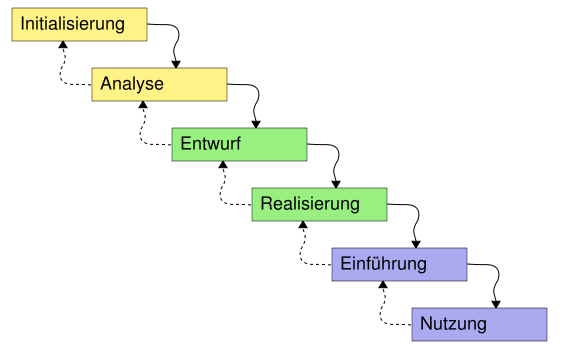
\includegraphics[scale=0.35]{567px-Wasserfallmodell.png}
\end{figure}
\footnote{Wasserfallmodell mit Rücksprung, Bild-Quelle: http://upload.wikimedia.org/wikipedia/commons/thumb/e/e5/Wasserfallmodell.svg/567px-Wasserfallmodell.svg.png}

\section{Warum dieses Modell?}
Wir haben uns für das Wasserfallmodell mit Rücksprung entschieden, weil dieses Modell alle Phasen der Entwicklung klar abgrenzt und sich optimal auf einen professionellen Softwareentwicklungsvorgang abbilden lässt.
Dieses Modell ermöglicht eine klare Planung und Kontrolle unseres Softwareprojekts, da die Anforderungen stets die gleichen bleiben und der Umfang einigermaßen gut abschätzbar ist.\\

Für die erweiterte Version dieses Modells, nämlich mit Rücksprung, haben wir uns entschieden, um ein paar Nachteile dieses Modells auszuhebeln. Beispielsweise sind die klar voneinander abgegrenzten Phasen in der Realität oft nicht umsetzbar. Des weiteren sind wir somit flexibler gegenüber Änderungen.

\chapter{Definition}
Der MPD ist eine Client/Server-Architektur, in der die Clients und Server (MPD ist der Server)
über ein Netzwerk interagieren. MPD ist also nur die Hälfte der Gleichung. Zur Nutzung von 
MPD, muss ein MPD-Client (auch bekannt als MPD-Schnittstelle) installiert werden.
\section{Definition des MPD}
\begin{quote}
    Der Music Player Daemon (kurz MPD) ist ein Unix-Systemdienst, der das Abspielen von Musik auf 
    einem Computer ermöglicht. Er unterscheidet sich von gewöhnlichen Musik-Abspielprogrammen dadurch, 
    dass eine strikte Trennung von Benutzeroberfläche und Programmkern vorliegt. Dadurch ist die 
    grafische Benutzeroberfläche auswechselbar und auch eine Fernsteuerung des Programms über das 
    Netzwerk möglich. Die Schnittstelle zwischen Client und Server ist dabei offen dokumentiert und 
    der Music Player Daemon selbst freie und quelloffene Software.\ \\ \\
    Der MPD kann wegen seines geringen Ressourcenverbrauchs nicht nur auf Standartrechnern sondern 
    auch auf einem abgespeckten Netzwerkgerät mit Audioausgang betrieben werden und von allen Computern
    oder auch Mobiltelefonen / PDAs im Netzwerk ferngesteuert werden.\ \\ \\
    Es ist auch möglich den Daemon und den Client zur Fernsteuerung lokal auf dem gleichen Rechner
    zu betreiben, er fungiert dann als normaler Medienspieler, der jedoch von einer Vielzahl 
    unterschiedlicher Clients angesteuert werden kann, die sich in Oberflächengestaltung und Zusatzfunktionen
    unterscheiden. Mittlerweile existierten auch zahlreiche Clients, die eine Webschnittstelle bereitstellen.\ \\ \\
    Der MPD spielt die Audioformate Ogg Vorbis, FLAC, OggFLAC, MP2, MP3, MP4/AAC, MOD, Musepack und wave ab.
    Zudem können FLAC-, OggFLAC-, MP3- und OggVorbis-HTTP-Streams abgespielt werden. Die Schnittstelle kann
    auch ohne manuelle Konfigruation mit der Zeroconf-Technik angesteuert werden. Des Weiteren wird Replay
    Gain, Gapless Playback, Crossfading und das Einlesen von Metadaten aus ID3-Tags, Vorbis comments oder
    der MP4-Metadatenstruktur unterstützt.
    \footnote{Zitat aus: http://de.wikipedia.org/wiki/Music\_Player\_Daemon}
\end{quote}
\newpage
\subsection{Der MPD kann:}
\renewcommand{\labelitemi}{•}
\begin{itemize}
    \item Musik abspielen
    \item Musik kontrollieren und in Warteschlangen reihen 
    \item Musik Dateien dekodieren
    \item HTTP(Hyper Text Transfer Protocol) streamen
        \renewcommand{\labelitemi}{--}
        \begin{itemize}
            \item Eine HTTP-URL kann zur Warteschlange hinzugefügt oder direkt abgespielt werden.\\
        \end{itemize}
\end{itemize}

\subsection{Der MPD kann nicht:}
\begin{itemize}
    \item Album-Cover speichern
    \item Funktionen eines Equalizers bereitstellen
    \item Musik Taggen (Informationen aus dem Web suchen)
    \item Text für Playlist-Dateien parsen
    \item Statistische Auswertungen machen
    \item Musik visualisieren
    \item Funktionen eines Remote-File-Servers bereitstellen
    \item Funktionen eines Video-Servers bereitstellen
\end{itemize}
\section{Definiton des MPD-Client}
Der Music Player Daemon Client ist nun die Schnittstelle zum MPD. Über diesen Client kann der MPD
gesteuert werden. Es gibt viele verschiedene Clients mit unterschiedlichsten Funktionen, da der 
Client nicht auf den Funktionsumfang des MPD begrenzt ist. Das heißt im Klartext, dass der Client
zwar nur die Funktionen über das Netzwerk steuern kann, die vom MPD implementiert sind aber nicht, 
dass er deshalb auch keine lokalen Dienste bzw. Funktionen anwenden kann. So kann ein Client 
beispielsweise alle Funktionen lokal implementieren, die unter dem Punkt \"3.1.2 Der MPD kann nicht:\" 
erwähnt wurden.
\newpage
\section{Grafische Übersicht}
\begin{figure}[h]
    \centering
    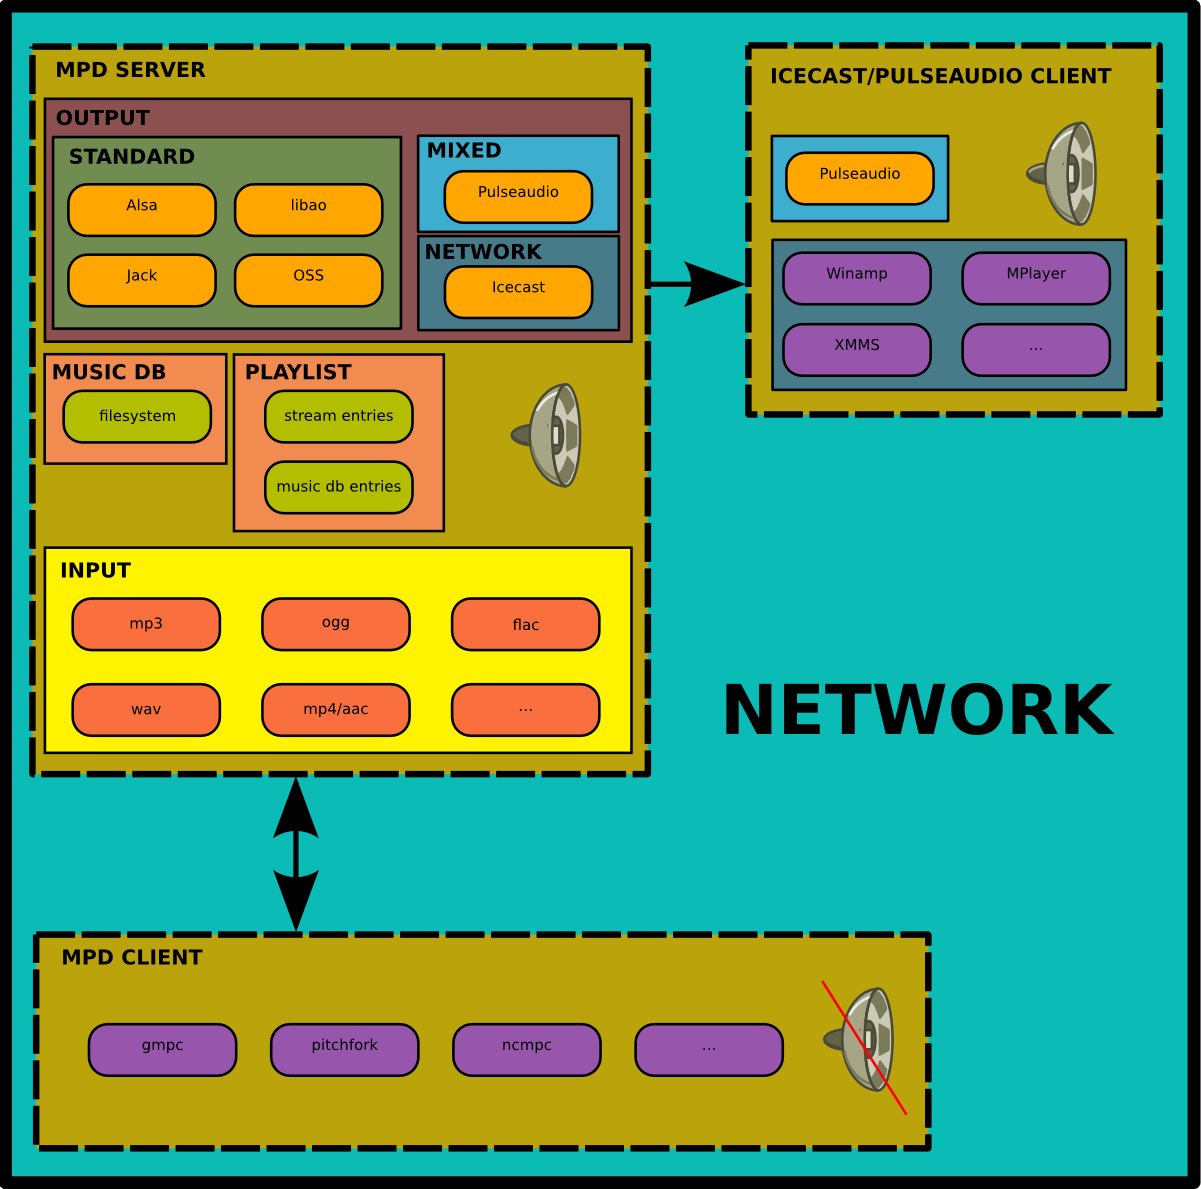
\includegraphics[scale=0.6]{Mpd-overview.png}
\end{figure}
\footnote{Bild-Quelle: http://images.wikia.com/mpd/images/6/68/Mpd-overview.png}
Der MPD-Server bekommt als Input mp3, ogg, flac, wav, mp4/aac,... Musik-Dateien die entweder in einer
Musik-Datenbank oder in Playlisten gespeichert sind. Der Standardoutput des MPD ist Alsa, libao, jack 
oder OSS, die Musik kann aber auch über einen Icecast oder Pulseaudio Clienten ausgegeben werden.
Der MPD-Client steuert den MPD-Server und hat selbst keinen Audio-Output.

\chapter{Anforderungen}

\section{Anforderungen aus Entwicklersicht}

\renewcommand{\labelitemi}{•}
\begin{itemize}
	\item Testfreundliche Implementierung für Prototypen
	\item Plug-In-Freundlichkeit
	\item Menschlich lesbare Configs
	\item Modular und Plattform-unabhängig
	\item Model-View-Controller
\end{itemize}

\section{Anforderungen aus Anwendersicht}

\begin{itemize}
	\item Standartfunktionen eines Music-Players
	\item Benutzerfreundlichkeit
	\item Grafische Oberfläche
	\item Playlisten erstellen und abspielen
	\item Musik favorisieren
	\item Recently-Played Funktion
	\item Dynamische Playlist
	\item Band-Informationen aus dem Internet	
\end{itemize}
\chapter{Funktionen des MPD-Client}

\section{MUSS für unseren MPD-Client}

\renewcommand{\labelitemi}{•}
\begin{itemize}
	\item Standartfunktion eines Music-Palyers (Abspielen, Skippen,...)
	\item Update-Funktion (...)
	\item Connection-Manager (Server-Client connection)
	\item Profil basierend (Configs und Playlists einem Benutzer zuordnen)
\end{itemize}

\section{KANN für unseren MPD-Client}
\begin{itemize}
	\item Songinformationen und Lyrics aus dem Internet
	\item Sortierfunktion (Interpret, Album, Titel, Genre)
	\item Playlist-Verwaltung
\end{itemize}

:::::::::HIER BEGRÜNDUNG WARUM WIR WAS IMPLEMENTIERT HABEN UND WAS WIR NICHT IMPLEMENTIERT HABEN MIT BEGRÜNDUNG::::::::
\chapter{Abhängigkeiten}

\section{Allgemeine Abhängigkeiten}

\renewcommand{\labelitemi}{•}
\begin{itemize}
	\item gtkmm-3.0
	\item libmpdclient
	\item libglyr
\end{itemize}

\section{Entwicklungsabhängigkeiten}
\begin{itemize}
	\item git (Versionsverwaltung)
	\renewcommand{\labelitemi}{--}
	\begin{itemize}
		\item git commit -a -m ("'Commit-Message"' Übertragen)
		\item git push (Änderungen auf den Github-Server laden)
		\item git pull (Änderungen von dem Github-Server laden)
	\end{itemize}
	\renewcommand{\labelitemi}{•}
	\item cmake (Buildsystem)
	\renewcommand{\labelitemi}{--}
	\begin{itemize}
		\item cmake . (Buildfiles erstellen)
		\item make (Kompilieren)
		\item sudo make install (Installieren)
	\end{itemize}
	\renewcommand{\labelitemi}{•}
	\item Editor nach Wahl (gVim, nano, Codeblocks, etc)
	\item Glade (Oberflächendesigner)
	\renewcommand{\labelitemi}{--}
	\begin{itemize}
		\item Erstellt ein XML File, kann von gtk geladen werden.
		\item Callbacks und Signale müssen im Code gehandelt werden.
	\end{itemize}
	\renewcommand{\labelitemi}{•}
	\item Primäre Entwicklerplattform: Linux
\end{itemize}

BEGRÜNDUNG!!!
\chapter{Programmierrichtlinien}

\renewcommand{\labelitemi}{•}
\begin{itemize}
	\item Programmiersprache C/C++
	\item Allman-Stil: http://de.wikipedia.org/wiki/Einr%C3%BCckungsstil#Allman_.2F_BSD_.2F_.E2.80.9EEast_Coast.E2.80.9C 
	\item Tabstop sind 4 Leerzeichen
	\item Striktes Prototyping
	\item Keine globalen Variablen
	\item Sinnvolle Variablenbenennung, Lowercase
	\item Klassenmethoden nur in Ausnahmen bzw. nur mit guten Gründen
	\item Valgrind darf keine Laufzeitfehler bringen, auch keine Memory Leaks.
	\item Camelcase bei Objektnamen, C-Style bei Funktionsnamen
	\item Modulare Gestaltung - Keinen GUI Code mit FeatureCode misschen
	\item "'make"' sollte auch keine Warnings ausgeben, die man leicht vermeiden 
könnte
	\item Testfälle pro Klasse 
	\item Doxygen für Dokumentation des Quelltextes
\end{itemize}


\end{document}
